\LARGE{ \textbf {Лекция №3}}\\
\Large{ \textbf {Сложение чисел с использованием дополнительного и обратных кодов.}}


В теории цифровых автоматов доказывается, что сумма обратных (дополнительных) кодов чисел есть обратный(дополнительный) от результата.\\
Замечание:\\
Теорема справедлива если отсутсвует переполнение разрядной сетки.\\

\Large{ \textbf {Сумматор дополнительных кодов.}} \\
Складывание - складываются все разряды кодов включая знаковые. Если возникает перенос из знакового разряда, то он отбрасывается.
Дополнительный код.\\
$
A = \quad 0.1000 \\
B = -0.0111 \\
A_{dop} = 0.1000 \\
+ \\
B_{dop} = 1.1001 \\
=\\
C_{dop} = 0.0001
$\\
----------------------------------\\
$
A = \quad 0.0100 \\
B =-0.1000  \\
A_{dop} = 0.0100  \\
+  \\
B_{dop} = 1.1000 \\
=  \\
C_{dop} = 1.1100
$\\
----------------------------------\\
$
A =-0.0011 \\
B =-0.0100  \\
A_{dop} = 1.1101  \\
+  \\
B_{dop} = 1.1100 \\
=  \\
C_{dop} = 11.1001  \\
$
Сумматор обратного кода.\\
При суммирований обратных кодов чисел в случае возникновения переноса из знакового разряда единицу переноса не отбрасывают, а ее добавляют в младший разряд кода результата, тем самым происходит циклический перенос.\\
Обратный код.\\
$
A =\quad 0.0011 \\
B =-0.1100  \\
A_{obr} = 0.0011  \\
+  \\
B_{obr} = 1.0011 \\
=  \\
C_{obr} = 1.0110
$\\
----------------------------------\\
$
A =\quad 0.1000 \\
B =-0.0100  \\
A_{obr} = 0.1000  \\
+  \\
B_{obr} = 1.1011 \\
=  \\
10.1011 \\
+\\
0.0001\\
C_{obr} = 0.0100  \\
$
При сложении дополнительных и обратных кодов может произойти переполнение, то есть получится сумма требующая для своего представления на один разряд больше по сравнению с разрядной сеткой слагаемых.
Признаками переполнения являются
\begin{enumerate}
  \item Наличие переноса в знаковый разряд при отсутствии переноса из знакового разряда.
  \item Нет переноса в знаковый разряд, при наличии переноса из знакового разряда.
\end{enumerate}
Иногда для обнаружения используют модифицированные прямой,обратный и дополнительные коды.в этом случае для кодирования знака числа используют 2 разряда. $00 - ‘+’ , 11 - ‘-’$

\Large{ \textbf {Глава 2. Логические основы цифровых автоматов.}} \\

При проектировании цифровых систем в качестве математического аппарата используется булева алгебра.\\
УТОЧНИТЬ
Цель болевой алгебры - описание поведения и структуры логических схем.\\
Чтобы описать поведение логической схемы нужно выразить функцию $Y_i$ как функцию от $x$.\\
$F_i$ - логическая функция аргументами которой являются логические переменные.\\
Совокупность значений n переменных $x_1, x_2, x_n$ будем называть входным набором значений.\\
Входной набор - входной сигнал для нашей лог функции, а значение $Y_i$ является выходными сигналами.\\
В общем случае входные, выходные сигналы могут иметь различную физическую природу. Обычно за единицу принимают высокий уровень сигнала, а за 0 - низкий.\\
\Large{ \textbf {
Логические функции от 2 переменных используемые в схемотехнике.\\
Конъюнкция, логическое умножение, операция И, схема И.
.}} \\
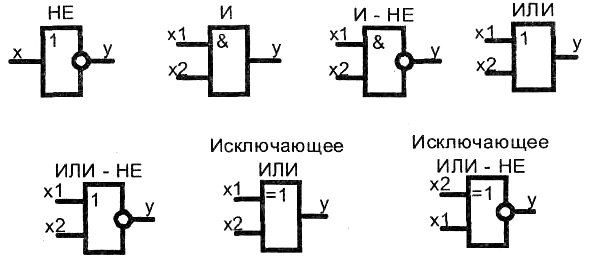
\includegraphics[width=\linewidth]{6} \\
И-НЕ:\\
Функция равна единице, когда хотя бы на одном из входов 0.\\
ИЛИ-НЕ:\\
Равна 0, когда хотя бы на одном из входов есть логическая единица.\\
Функция сложения по модулю 2, М2 , исключающее ИЛИ:\\
Функция неравнозначности.\\
Одно из основных понятий болевой алгебры логики это понятие функциональной полноты системы булевых функций.\\
Система булевых функция называется функционально полной, если на ее основе можно получить любую булеву функцию, используя лишь принцип суперпозиции.\\
Пример:
\begin{itemize}
  \item ИЛИ-НЕ
  \item И,ИЛИ,НЕ
  \item И-НЕ
\end{itemize}

Под принципом суперпозиции понимается возможность использовать результаты функций в качестве аргументов для других.\\
\Large{ \textbf {Аналитическое представление логических функций.}} \\

Булево выражение - формула представляющая сост из булевых констант и переменных связанных операциями и,или,не.\\
Порядок старшинства: НЕ,И,ИЛИ. Для изменения порядка используются скобки.\\
Пример 3
$$f(x_1 ,x_2 ,x_3)= (x_1 + \neg x_2) \cdot (\neg x_1 + x_3) + x_3 x_2 $$
Логическая схема которую можно полностью описать таблицами истинности или булевыми выражениями называется комбинационной схемой —КС.\\
В КС значение выходного сигнала полностью определятся значениями входного сигнала, в текущей момент времени.\\
Другой класс схем — это схемы с внутренней памятью называемыми последовательсные, в них значения выходных сигналов определяются не только текущими значениями сигналов но и их значениями в предыдущие моменты времени.\\
